%-------------------------------------------------------------------------------
% Autores: I. R. Pagnossin e Centro de Ensino e Pesquisa Aplicada.
%
% Este material é parte integrante do curso "Usando LaTeX; pensando em TeX" e é
% distribuido pelos autores segundo a licença Creative Commons 2.5 Brasil
% (atribuição/não-comercial/redistribuição segundo a mesma licença).
%
% This material is part of the course "Usando LaTeX; pensando em TeX".
% It is distributed according to the license Creative Commons 2.5 Brazil
% (attribution/non-comercial use/share alike the same license).
%-------------------------------------------------------------------------------
\newif\ifhandout
%\handouttrue  % Descomente se for para gerar a versão para IMPRESSÃO.
\handoutfalse % Descomente se for para gerar a versão para APRESENTAÇÃO

%-------------------------------------------------------------------------------
\ifhandout
  \documentclass[handout,10pt]{beamer}
  \mode<handout>
\else
	\documentclass[10pt,hyperref={pdfpagelabels=false}]{beamer}
	\mode<presentation>
\fi

	\usepackage[utf8]{inputenc}
	\usepackage{ae}	
	\usepackage[brazil]{babel}	
	\usepackage{graphicx}
	\usepackage{listings}
	\usepackage{tikz}
	\usepackage{amsmath}
	\usepackage[squaren]{SIunits}
	\usepackage{booktabs}
	\usepackage{fancybox}
	\usepackage{array}
	\usepackage{colortbl}
	
	\newsavebox{\mybox}
	\savebox{\mybox}{\LARGE$italico$}
	
	\usepackage{bookman}
	
	\ifhandout
		\usepackage{pgfpages}
		\pgfpagesuselayout{2 on 1}[a4paper,border shrink=5mm]
	\fi

	% Bibliotecas TikZ e PGF necessárias
	\usetikzlibrary{shapes.symbols}
	\usetikzlibrary{calc}
	\usepgflibrary{shapes.misc}
	
	% Configurações pessoais
	% Configurações personalizadas do código LaTeX.	
\lstnewenvironment{LaTeXcode}{
	\setlength{\abovecaptionskip}{0pt}	
	\lstset{language=[LaTeX]TeX}
	\lstset{%
		basicstyle=\footnotesize\ttfamily,  % Global
		keywordstyle=\color{blue}\bfseries, % Comandos
		identifierstyle=,                   % Texto
		stringstyle=,                       % Strings 
		commentstyle=\color{gray},          % Comentários
		showstringspaces=false,             % Espaços
		rulecolor=\color{gray},             % Linha da caixa
	}
	\lstset{emph={setlength,includegraphics,psfrag,subfigure},emphstyle={\color{blue}\bfseries}}
}% Abrindo o ambiente.
{}% Fechando o ambiente.
	
\newcommand{\digite}[1]{{\fontfamily{cmss}\fontseries{bx}\selectfont#1}}	
\newcommand{\cs}[1]{{\normalfont\textbackslash\color{blue!50!black}#1}}
\newcommand{\pkg}[1]{{\normalfont\sffamily\color{orange}#1}}
\newcommand{\env}[1]{{\normalfont\sffamily\color{green!50!black}#1}}
\let\comando=\cs
\let\package=\pkg
\let\ambiente=\env
\newcommand{\foreign}[1]{{\textsl{#1}}}


	\newcounter{exercicio}	
	\newenvironment{exercicio}{%
		\refstepcounter{exercicio}%
		\penalty-200
		\noindent\colorbox{blue!60!black}{\makebox[\columnwidth-\fboxsep*2][c]{\textbf{\color{white}Exercício~\theexercicio}}}\smallskip
	}{\par\medskip}
		

\newcommand{\bibtex}{\textsc{Bib}\TeX}

\newenvironment<>{atividade}[1]{%
\begin{actionenv}#2%
\begin{exampleblock}{{Atividade #1}}%
}
{%
\end{exampleblock}%
\end{actionenv}%
}


	% Path das figuras, relativo a esta pasta.
	\graphicspath{{../arquivos_comuns/figuras/}{./figuras/}}

	% Modelo da apresentação	
	\usetheme{Frankfurt}
	\usefonttheme{serif,structurebold}
	\setbeamercovered{transparent}		
		
	% Metadados do arquivo PDF.
	\hypersetup{
		pdftitle={Comprimentos e comprimentos elásticos},
		pdfauthor={Dr. Ivan R. Pagnossin},
		pdfsubject={LaTeX},
		pdfkeywords={TeX,LaTeX}
	}

	% Título, autores e instituição.
	\title{Comprimentos}
	\subtitle{e comprimentos elásticos}
	\author{\textbf{Prof.:} Ivan R. Pagnossin \and \textbf{Tutora:} Juliana Giordano}
	\institute{%
		Coordenadoria de Tecnologia da Informação\\
		Centro de Ensino e Pesquisa Aplicada}
	\logo{
\includegraphics[width=0.25\textwidth]{LogotipoCursoLaTeX_v3_pequeno}}
	\date{}
	
	\newsavebox{\minhacaixa}
	\savebox{\minhacaixa}{%
		\setlength{\parindent}{1cm}
		\begin{tikzpicture}
			\node (linha1) at (\parindent,0) {Primeira linha de texto\dots};
			\node (linha2) at (0,-\baselineskip) {Segunda linha de texto\dots};
			\draw [thin,red!70] let \p1 = (linha1.base) in (+15mm,\y1) -- (+40mm,\y1);
			\draw [thin,red!70] let \p2 = (linha2.base) in (+15mm,\y2) -- (+40mm,\y2);
			
			\draw [<->] let \p1 = (linha1.base), \p2 = (linha2.base) in (+39mm,\y1) -- (+39mm,\y2);
			\draw [thin,red!70] let \p1 = (linha1.west),
			                        \p2 = (linha2.west),
			                        \p3 = (linha1.base) in (\x2+1mm,\y3) -- (\x2+1mm,\y3+5mm)
			                                               (\x1+1mm,\y3) -- (\x1+1mm,\y3+5mm);
			\draw [<->] let \p1 = (linha1.west),
			                \p2 = (linha2.west),
			                \p3 = (linha1.base) in (\x1+1mm,\y3+4mm) -- (\x2+1mm,\y3+4mm);
			\node [right] at (40mm,-0.5\baselineskip-0.7ex) {{\small\ttfamily \textbackslash\textcolor{blue}{baselineskip}}};
			\node at (-18mm,6mm) {{\small\ttfamily \textbackslash\textcolor{blue}{parindent}}};
		\end{tikzpicture}}
\begin{document}


%-------------------------------------------------------------------
\begin{frame}[c,label=titulo]
	\centering	
	
	
\includegraphics[width=0.8\textwidth]{LogotipoCursoLaTeX_v2}

	\titlepage
\end{frame}
%-------------------------------------------------------------------
\logo{} % <-- O logotipo não aparecerá mais a partir daqui.
\setbeamertemplate{background canvas}{%
		
\includegraphics[width=\paperwidth,height=\paperheight,keepaspectratio=false]{leao-pensador-wattermark.png}
}
%-------------------------------------------------------------------
\section{Comprimentos}
\subsection{Representação no \LaTeX}
\begin{frame}
	\frametitle{Comprimentos}
	\framesubtitle{Representação no \LaTeX}
	
	\begin{block}<1->{}
		\centering
		{\bfseries comprimento: valor numérico + unidade}
		
		\medskip
		
		\texttt{3.1 mm}\qquad \texttt{-1ex}\qquad \texttt{0in}\qquad \texttt{+6,5  pt}		
	\end{block}
	
	\vspace*{\stretch{1}}
	
	\begin{itemize}
		\item<1-> Valor numérico
		\begin{itemize}
			\item<2-> deve ser positivo, negativo ou nulo
			\item<3-> pode ter ponto, vírgula ou nenhum deles
		\end{itemize}
		
		\item<1-> Unidade \uncover<4->{deve ser uma das seguintes:}
		\begin{itemize}
			\item<4-> \milli\metre
			\item<5-> \centi\metre
			\item<6-> in \onslide<6>{(\foreign{inch} ou polegada)}
			\item<7-> pt \onslide<7>{(\foreign{point} ou ponto)}
			\item<8-> \alert<11>{em} \onslide<8>{(largura do ``M'' maiúsculo)}
			\item<9-> \alert<11>{ex} \onslide<9>{(altura do ``x'' minúsculo)}\\
								\hyperlink{comprimentos}{\color{blue}\underline{etc}}
		\end{itemize}
	\end{itemize}
	
	\vspace*{\stretch{1}}
	
	\begin{center}
		\footnotesize
		\uncover<10->{\textbf{obs.:} a unidade deve estar presente mesmo que o valor numérico seja zero}\\
		\uncover<10->{\textbf{obs.:} o espaço entre o valor numérico e a unidade é opcional}
	\end{center}
	
\end{frame}
%-------------------------------------------------------------------
\subsection{Alterando um comprimento existente}
\begin{frame}[fragile]
	\frametitle{Alterando um comprimento existente}
	
	\begin{block}<1->{}
		\centering
		\verb|\setlength{\|\textit{nome}\verb|}{|\textit{comprimento}\verb|}|
	\end{block}
	
	\vspace*{\stretch{1}}
	
	\begin{uncoverenv}<2->
		\begin{center}
			\usebox{\minhacaixa}
		\end{center}
	\end{uncoverenv}
	
	\vspace*{\stretch{1}}
	
	\begin{atividade}<3->{1}
		\begin{LaTeXcode}
			\setlength{\parindent}{2cm}
		\end{LaTeXcode}
	\end{atividade}
	
	\vspace*{\stretch{1}}
	
	\begin{atividade}<4->{2}
		\begin{LaTeXcode}
			\setlength{\baselineskip}{-24pt}
			\setlength{\lineskip}{-24pt}
		\end{LaTeXcode}
	\end{atividade}
\end{frame}
%-------------------------------------------------------------------
\subsection{Dimensões do documento}
\begin{frame}
	\frametitle{Dimensões do documento}
	\framesubtitle{\textcolor{yellow}{Atividades 3A e 3B}}
	
	\begin{columns}
		\column[c]{0.5\textwidth}
			\small
			\begin{enumerate}
			\item $\unit{1}{in} + \text{\cs{hoffset}}$
			\item $\unit{1}{in} + \text{\cs{voffset}}$
			\item \cs{oddsidemargin} {\scriptsize(pp. ímpares)}\\
			      \cs{evensidemargin} {\scriptsize(pp. pares)}
			\item \cs{topmargin}
			\item \cs{headheight}
			\item \cs{headsep}
			\item \cs{textheight}
			\item \cs{textwidth}
			\item \cs{marginparsep}
			\item \cs{marginparwidth}
			\item \cs{footskip}
			\item \cs{paperwidth}
			\item \cs{paperheight}
			\end{enumerate}
			
		\column[c]{0.45\textwidth}
			\centering
			\raisebox{-\height}{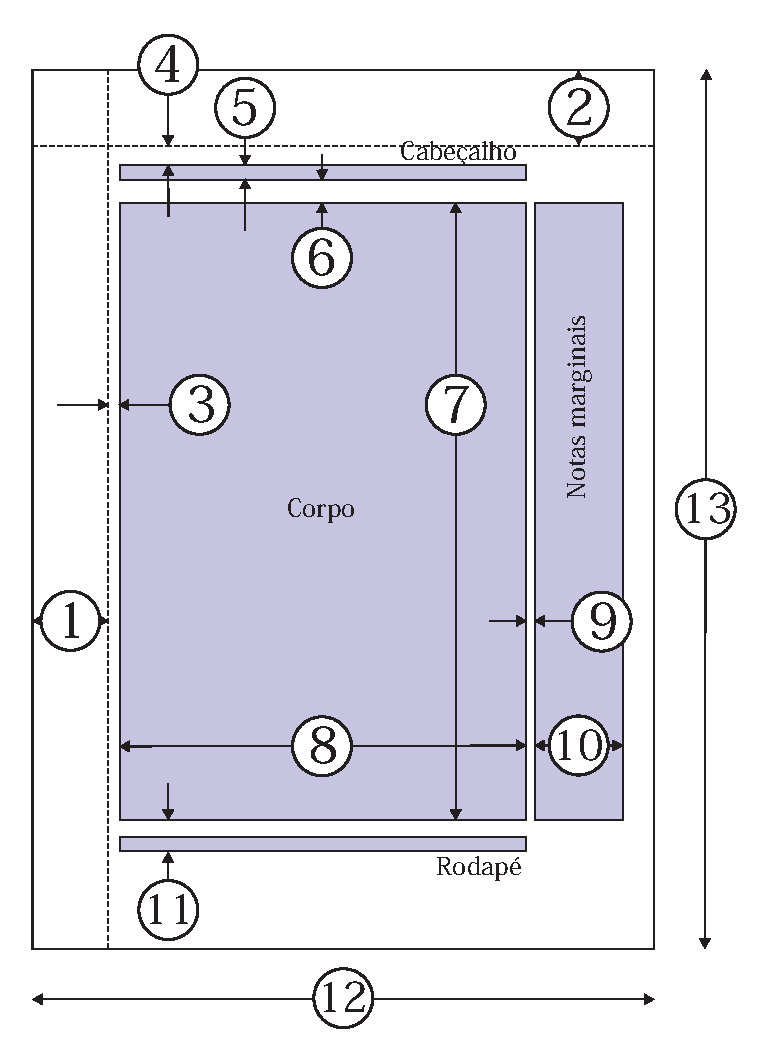
\includegraphics[width=1.1\textwidth,trim=10 10 10 10]{Layout_A4_article}}
	\end{columns}
	
\end{frame}
%-------------------------------------------------------------------
\subsection{Espaços horizontais}
\begin{frame}[fragile]
	\frametitle{Espaços horizontais}
	
	\begin{block}<1->{\textcolor{white}{\textbackslash hspace}: \foreign{horizontal space}}
		\centering
		\verb|\hspace {|\textit{comprimento}\verb|}|\\
		\verb|\hspace*{|\textit{comprimento}\verb|}|
	\end{block}
	
	\vspace*{\stretch{1}}
	
	\begin{atividade}<2->{4}
		A diferença entre \cs{hspace} e \cs{hspace*}:
		\begin{LaTeXcode}		
			\noindent\hspace{2cm}texto\\
			         \hspace{2cm}texto   % <-- Precisa de \hspace*
		\end{LaTeXcode}

		\medskip

		Cuidado com espaços espúrios:
		\begin{LaTeXcode}
			Espaço\hspace{1cm}horizontal.\par			
			Espaço \hspace{1cm}horizontal.\par			
			Espaço \hspace{1cm} horizontal.
		\end{LaTeXcode}
	\end{atividade}
		
\end{frame}
%-------------------------------------------------------------------
\subsection{Espaços verticais}
\begin{frame}[fragile]
	\frametitle{Espaços verticais}
	
	\begin{block}<1->{\textcolor{white}{\textbackslash vspace}: \foreign{vertical space}}
		\centering
		\verb|\vspace {|\textit{comprimento}\verb|}|\\
		\verb|\vspace*{|\textit{comprimento}\verb|}|
	\end{block}
	
	\vspace*{\stretch{1}}
	
	\begin{atividade}<2->{5}
		\begin{LaTeXcode}
			A primeira linha da página\dots
			
			\vspace{1cm}
			
			A segunda linha da página\dots\\[1cm]
			A terceira linha (2\textordmasculine\ parágrafo ainda).
			
			\newpage % <-- Mudança de página
	
			\vspace{10cm} % <-- Precisa de \vspace*
			Esta linha está mais ou menos no centro da página?
		\end{LaTeXcode}
	\end{atividade}
	
	\vspace*{\stretch{1}}
	
	\begin{center}
		\begin{uncoverenv}<3->
			\textbf{obs.:} o comando \verb|\\| \emph{não} causa mudança de parágrafo!
		\end{uncoverenv}
	\end{center}			
\end{frame}
%-------------------------------------------------------------------
\subsection{Comprimentos elásticos}
\begin{frame}[fragile]
	\frametitle{Comprimentos elásticos (\LaTeX)}
	\framesubtitle{ou cola (\TeX)}

	\begin{block}<1->{}
		\centering
		{\bfseries comp. natural \texttt{\color{blue}plus} comp. \texttt{\color{red}minus} comp.}
		
		\texttt{12pt plus5pt minus 1cm}\qquad \texttt{-1cm minus 7mm}
	\end{block}
	
	\vspace*{\stretch{1}}
	
	\begin{block}<4-6>{Exercício 1\hspace*{\stretch{1}}\hyperlink{respostas}{\footnotesize\textbf{(resposta)}}}
		Dada a cola \texttt{20pt plus5pt minus 5pt}, responda:
		\begin{enumerate}
			\item<4-> Qual é o seu comprimento natural?
			\item<5-> Qual é o seu comprimento máximo?
			\item<6-> Qual é o seu comprimento mínimo?
		\end{enumerate}
	\end{block}
	
	\vspace*{\stretch{1}}
	
	\begin{atividade}<7->{6}
		\begin{LaTeXcode}
			\noindent texto\hspace{\textwidth minus 0.5\textwidth}texto
		\end{LaTeXcode}
	\end{atividade}
	
	\vspace*{\stretch{1}}
	
	\begin{center}\footnotesize
		\uncover<2->{\textbf{obs.:} o espaço \emph{após} \texttt{plus}/\texttt{minus} é opcional}\\
		\uncover<3->{\textbf{obs.:} as \emph{unidades} de \texttt{plus} e \texttt{minus} não precisam ser iguais}
	\end{center}
	
\end{frame}
%-------------------------------------------------------------------
\begin{frame}[fragile]
	\frametitle{Comprimentos elásticos}
	\framesubtitle{\textbackslash fill, \textbackslash hfill e \textbackslash vfill}
	
	\begin{block}<1->{\textbackslash fill: \emph{comprimento} nulo e arbitrariamente extensível}
		\centering
		\(\verb|\fill| = \verb|0pt plus |\infty\)
	\end{block}
	
	\vspace*{-\baselineskip}
	
	\begin{columns}
		\column[t]{0.47\textwidth}
		
		\begin{block}<2->{\emph{Espaço} horizontal}
			\centering
			\(\verb|\hfill| = \verb|\hspace{\fill}|\)
		\end{block}
		
		\begin{atividade}<2->{7}
			\begin{LaTeXcode}
				\hfill texto
				
				texto\hfill
			
				texto\hfill texto	
			\end{LaTeXcode}
		\end{atividade}	
	
		\column[t]{0.47\textwidth}
		
		\begin{block}<3->{\emph{Espaço} vertical}
			\centering
			\(\verb|\vfill| = \verb|\vspace{\fill}|\)
		\end{block}
		
		\begin{atividade}<3->{7}
			\begin{LaTeXcode}
				Uma linha no início da página.
				
				\vfill
			
				Uma linha no final da página.
			\end{LaTeXcode}
		\end{atividade}
	\end{columns}

	\vspace*{\stretch{1}}

	\begin{center}
		\uncover<4->{\textbf{Atenção:} \cs{fill} é um comprimento elástico;\\\cs{hfill} e \cs{vfill} são \emph{espaços} (de comprimento elástico).}
	\end{center}
	
\end{frame}
%-------------------------------------------------------------------
\subsection{Comprimentos personalizados}
\begin{frame}[fragile]
	\frametitle{Comprimentos personalizados}
	
	\begin{block}<1->{}
		\centering
		\verb|\newlength{|\textit{nome do comprimento}\verb|}|
	\end{block}

	\vspace*{\stretch{1}}

	\begin{atividade}<2->{8}
		\begin{LaTeXcode}
			\newlength{\meucomp}
			\setlength{\meucomp}{\textwidth minus 0.5\textwidth}
			
			\noindent texto\hspace{\meucomp}texto
		\end{LaTeXcode}
	\end{atividade}
	
	\vspace*{\stretch{1}}
	
	\begin{block}<3->{Exercício 2\hspace*{\stretch{1}}\hyperlink{respostas}{\footnotesize\textbf{(resposta)}}}
		Construa um texto com três parágrafos de tal modo que a endentação do segundo seja igual a \unit{5}{\centi\metre} e a do terceiro, igual ao dobro da do primeiro.
		
		\medskip
		
		\footnotesize\textbf{dica:} salve o comprimento \cs{parindent} antes de alterá-lo.
	\end{block}
\end{frame}
%-------------------------------------------------------------------
\newlength{\mylength}
\subsection{Espaços especiais}
\begin{frame}[fragile]
	\frametitle{Espaços especiais}
	
	\centering
	
	\begin{tabular}{l!{\(=\)}r@{}ll}
		\multicolumn{4}{c}{\cellcolor{red!50!black}\textbf{\textcolor{white}{Espaços horizontais}}}\\
		\verb|\enspace|&                    & \unit{1}{en} & \settowidth{\mylength}{\enspace}\rule{\mylength}{2pt}  \\
		\verb|\quad|  &                    &\verb|\normalsize| ou \unit{1}{em} & \settowidth{\mylength}{\quad}\rule{\mylength}{2pt}  \\
		\verb|\qquad| & \(2\)              &\verb|\quad|       & \settowidth{\mylength}{\qquad}\rule{\mylength}{2pt} \\
		\verb|\!|     & \(-\frac{3}{18}\)  &\verb|\quad|       & \settowidth{\mylength}{\!}\rule{-\mylength}{2pt}    \\
		\verb|\,|     & \(+\frac{3}{18}\)  &\verb|\quad|       & \settowidth{\mylength}{\,}\rule{\mylength}{2pt}     \\
		\verb|\:|     & \(+\frac{4}{18}\)  &\verb|\quad|       & \settowidth{\mylength}{\:}\rule{\mylength}{2pt}     \\
		\verb|\;|     & \(+\frac{5}{18}\)  &\verb|\quad|       & \settowidth{\mylength}{\;}\rule{\mylength}{2pt}\\
		\verb|\hfill| & &\verb|\hspace{\fill}| (\(\unit{0}{pt} + \infty\))  \\[\medskipamount]
		\multicolumn{4}{c}{\cellcolor{red!50!black}\textbf{\textcolor{white}{Espaços verticais}}}\\		
		\verb|\smallskip| & &\(\unit{4}{pt} \pm \unit{1}{pt}\) &  \rule{\smallskipamount}{2pt} \\
		\verb|\medskip|   & &\(\unit{6}{pt} \pm \unit{2}{pt}\) &  \rule{\medskipamount}{2pt} \\
		\verb|\bigskip|   & &\(\unit{12}{pt} \pm \unit{4}{pt}\) &  \rule{\bigskipamount}{2pt} \\
		\verb|\vfill| & &\verb|\vspace{\fill}| (\(\unit{0}{pt} + \infty\))  \\
		\bottomrule[0.1pt]
	\end{tabular}
	
	\vspace*{\stretch{1}}
	
	\small
	\begin{tabbing}
		\textbf{obs.1:} \=$\verb|\quad|/18$ é o valor de uma \emph{unidade matemática} (mu).\\
		\textbf{obs.2:} \>os comprimentos acima podem ser utilizados tanto no modo\+\\parágrafo quanto no matemático, exceto \verb|\vfill|: só no texto.
	\end{tabbing}
		
\end{frame}
%-------------------------------------------------------------------
{
	\logo{
\includegraphics[width=0.25\textwidth]{LogotipoCursoLaTeX_v3_pequeno}}
	\setbeamertemplate{background canvas}{}
	\againframe{titulo} % Reapresenta a página inicial.
}
%-------------------------------------------------------------------
%-------------------------------------------------------------------
%-------------------------------------------------------------------
\section{Apêndice}
\subsection{Respostas}
\begin{frame}[fragile,label=respostas]
	\frametitle{Respostas}
	\scriptsize
	
	\begin{enumerate}
	\item Comprimento natural: \unit{20}{pt}\\
	      Comprimento máximo: \unit{25}{pt}\\
	      Comprimento mínimo: \unit{15}{pt}
	      
	\item Nesta resposta os parágrafos foram gerados com o comando \cs{lipsum},\\do pacote \pkg{lipsum}:
	
		\begin{LaTeXcode}
		\newlength{\meucomp}
		
		\setlength{\meucomp}{2\parindent}
		\lipsum[1] % 1o parágrafo
		
		\setlength{\parindent}{5 cm}
		\lipsum[2] % 2o parágrafo
		
		\setlength{\parindent}{\meucomp}
		\lipsum[3] % 3o parágrafo
		\end{LaTeXcode}
	\end{enumerate}

\end{frame}
%-------------------------------------------------------------------
\subsection{Unidades de comprimento permitidas no \TeX}
\begin{frame}[label=comprimentos]
	\frametitle{Unidades de comprimento permitidas no \TeX}

	\begin{tabbing}
		A unidade deve ser: \=\milli\metre \+\\
		                      sp (\foreign{scaled point}) \=\kill
		                      \centi\metre \\
		                      in (\foreign{inch})         \>\(=\unit{25,4}{\milli\metre}\) \\
		                      pt (\foreign{point})        \>\(=\unit{0,35}{\milli\metre}\) \\		                        
		                      bp (\foreign{big point})    \>\(=\unit{1,00375}{pt}\) \\
		                      dd (\foreign{didot point})  \>\(=\unit{1,07}{pt}\) \\
		                      pc (\foreign{pica})         \>\(=\unit{12}{pt}\) \\
		                      cc (\foreign{cicero})       \>\(=\unit{12,84}{pt}\) \\
		                      sp (\foreign{scaled point}) \>\(\sim\unit{5,3}{\micro\metre}\) \\
		                      em                          \>\(=\text{Largura do ``M''}\) \\
		                      ex                          \>\(=\text{Altura do ``x''}\) \\
	\end{tabbing}
\end{frame}
\end{document}